\chapter{Forward Model in Electrical Source Imaging}
\label{ch:forward}

%%%%%%%%%%%%%%%%%%%%%%%%%%%%%%%%%%%%%%%%%%%%%%%%%%%%%%%%

%TODO: Better intro to the intro

%cite the review from Hllez\cite{hallez2007review}.

%%%%%%%%%%%%%%%%%%%%%%%%%%%%%%%%%%%%%%%%%%%%%%%%%%%%%%%%
%%%%%%%%%%%%%%%%%%%%%%%%%%%%%%%%%%%%%%%%%%%%%%%%%%%%%%%%

Electroencephalography (EEG) is a type of electrophysiological recording that uses electrodes, whose contact surface is in the order of 20 \si{mm^2}, placed on the subject's scalp.
%
The recording circuit is typically completed with a reference electrode at a `neutral' location, like the contra-lateral earlobe or the nose; another electrode can also be used, resulting in referential channels. 
%
%The effect of the reference electrode location may be neglected by re-referencing the recordings against the average.

In the century since the invention of the EEG machine, the simultaneous observation of behavioral data and EEG recordings has helped establish strong connections between specific EEG patterns and normal and pathological conditions.

The neural origin of electrical signals measured by EEG can be traced to the post-synaptic potentials in neurons' axons.
%
Although each individual neuron cannot produce an electric potential field large enough to be measured by the EEG electrodes at the scalp, the simultaneous firing of all the neurons in the brain is sufficient to produce the EEG measurements.

It is important to acknowledge that the EEG may also register events whose origin is not neural, referred to as artifacts. These include but are not limited to external electrical fields, eye movements, activity from facial muscles, and movement from the EEG electrodes —if they are not fixated adequately to the scalp or if the subject's movement is excessive.
%
This work does not discuss any methods for dealing with artifacts; the interested reader must refer to specialized manuals, for example, that from Fish and Spehlmann \cite{fisch1999fisch}.

In the absence of artifacts, either biological or instrumental, the EEG measurements are produced exclusively by brain activity.
%
The electric potential fields at the EEG scale, often called macro-scale fields, correspond to large groups of neurons that fire simultaneously and have a common physical orientation.
%
It is estimated that groups of neurons of at least 6 \si{mm^2} are required to produce activity measurable at the EEG scale.

\section{Electrical Source Imaging Framework}

Electrical Source Imaging (ESI), or Electrical Source Reconstruction, involves identifying the neural electrical sources responsible for the observed EEG.
%
ESI can be used to identify brain regions related to (and, in some cases, responsible for) the normal or pathological state under study.

For a review of ESI paradigms, see []. 
%
In this work, we perform ESI under the distributed dipole paradigm: the current density field produced by neuronal activity is approximated by a finite set of electrical dipoles whose location is known --on a grid that covers the brain region of interest-- and whose magnitude is to be determined. 

This paradigm can be justified formally as a discretized multi-pole expansion of order 2 (using dipoles) of the current density field; this approximation is sufficient to explain measurements obtained 1 mm or farther from the electrical sources \cite{nunez2019multi}.

ESI with distributed dipoles aims to produce a representative set of dipoles that will produce an equivalent current density of the real neurons at the EEG scale.
%
This paradigm is considered to be non-parametric in the sense that it is agnostic to the number and extent of the electric sources. 
%
Since an area with no discernible activity will produce a group of dipoles with a magnitude close to zero, this paradigm is considered robust to model misidentification.

When interpreting the results obtained from ESI, one should be aware of the limitations inherited from EEG.
%
For example, the lack of synchronization of time and direction of some active neuron patches may prevent them from producing an electric potential that can be measured by the EEG.
%
This silent activity can't be measured by ESI methods based on EEG data.

The task of performing ESI within the paradigm of distributed dipoles is an ill-posed inverse problem.

The `inverse problem' denomination is earned since the reciprocal problem is relatively more straightforward: constructing EEG recordings given the current density.
%
This problem is explored in Section \ref{sec:forward_derivation}, following that of Hallez et al. \cite{hallez2007review}.

The `ill-posed' denomination is earned since, given the data from EEG recordings, the current density is not uniquely defined.
%
In Chapter \ref{ch:review}, we review some methods used to solve this problem, while in Chapter \ref{ch:review}, we propose a novel method for this purpose.

%%%%%%%%%%%%%%%%%%%%%%%%%%%%%%%%%%%%%%%%%%%%%%%%%%%%%%%%
%%%%%%%%%%%%%%%%%%%%%%%%%%%%%%%%%%%%%%%%%%%%%%%%%%%%%%%%

\section{Derivation of the Forward Problem}
\label{sec:forward_derivation}

From a Physics framework, we can describe that EEG sensors measure the electric scalar potential field, $V: \R^3 \rightarrow \R$, at a finite set of points in space, $\sa_{1}, \sa_2, \dots, \sa_M \in \R^3$. 
%
Thus, $V(\sa_m)$ represents the measurement from the $m$-th electrode.

We assume that the electric scalar potential field is caused by a finite number of dipoles with known locations, ${\dd_1, \dd_2, \dots, \dd_N \in \R^3}$, and whose momentum, $\mm_1, \mm_2, \dots \mm_N \in \R$, are to be determined.

We first construct a model for a single sensor and a single dipole with unit moment. 
%
The full model will be constructed later by superposing multiple copies of this base model.

Under these circumstances, we consider the electric field, $E: \R^3 \rightarrow \R^3$, and the current density field, $K: \R^3 \rightarrow \R^3$,
\begin{align}
E &= - \nabla V
\\
K &= \sigma E = - \sigma \nabla V
\label{eq:model1}
\end{align}
with $\sigma: \R^3 \rightarrow \R^{3\times 3}$ the position-dependent conductivity tensor. 
%
In the isotropic case, we assume
$\sigma(\rr) = \kappa \id_3$
for all $\rr$, where $\kappa>0$ is the constant conductivity and $\id_3 \in \R^{3\times 3}$ is the identity matrix.

The current density field has the property that its divergence vanishes everywhere except near the dipole.
%
In more precise terms, the divergence of the current density field is defined as
\begin{equation}
\nabla \cdot K = \lim_{G(\rr) \rightarrow \sset{\rr}} \frac{1}{\text{vol}\ppar{G\ppar{\rr}}}
\oint_{\partial G(\rr)} K(\rr)\, dS
\label{eq:divK}
\end{equation}
with $G(\rr)\subset \R^3$ a set that contains $\rr$. 
%
The limit must be interpreted in a similar way as Riemann sums, in the sense that the limit is not affected by the selections of $G(\rr)$.

For the case of one single dipole, $\nabla \cdot K$ can be simplified,
\begin{equation}
\nabla \cdot K(\rr) = {\delta\ppar{\rr-\dd^+} - \delta\ppar{\rr-\dd^-}} =
\begin{cases}
+1, &\text{if } \rr=\dd^+ \\
-1, &\text{if } \rr=\dd^- \\
0, &\text{otherwise}.
\end{cases}
\label{eq:model2}
\end{equation}
where $\dd^-, \dd^+ \in \R^3$ are the dipole's electric sink and source positions, respectively. 
%
For ease of notation, we select $\dd^-$ and $\dd^+$ so that the dipole position, $\dd$, and momentum, $\mm$, satisfy the following
\begin{align}
    \dd &= \frac{1}{2}\spar{\dd^-+\dd^+} 
    \\
    \mm &= \spar{\dd^+-\dd^-}
\end{align}
%
Refer to figure \ref{fig:diagrams1} for a graphical summary of this construction.

\begin{figure}
\centering
%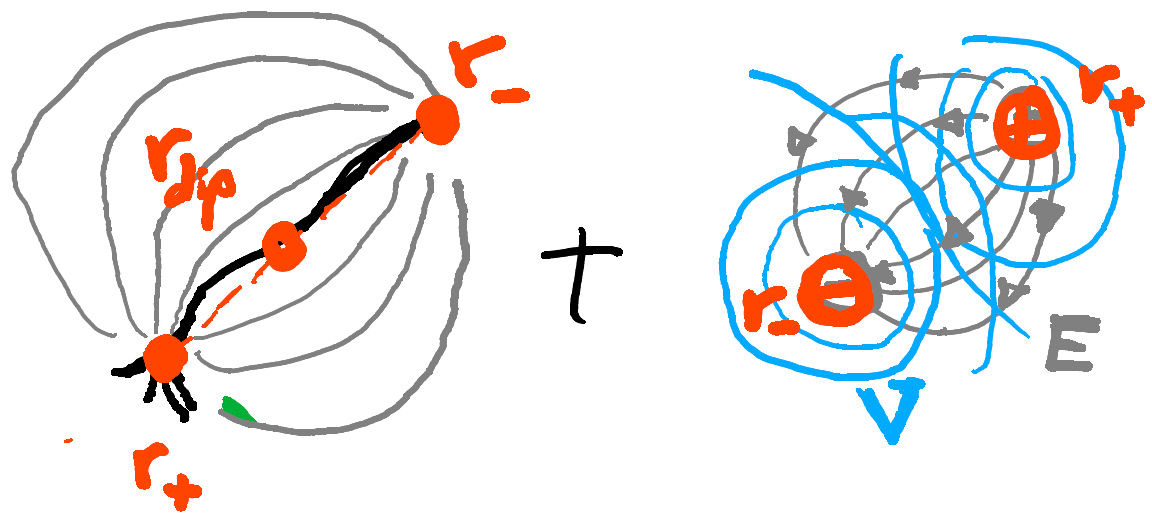
\includegraphics[width=0.4\linewidth]{./img_dev/nsNeuronDipole}
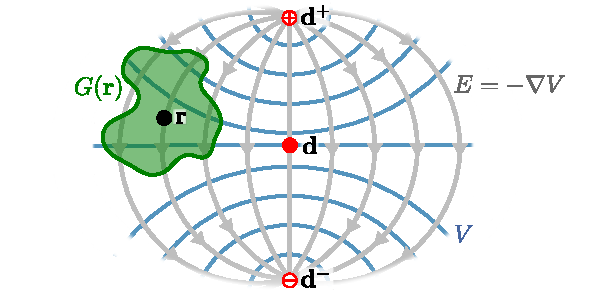
\includegraphics{./img/CurrDensField.pdf}
\caption{Visual representation of a single dipole with electric sink and source located at $\dd^-$ and $\dd^+$, respectively.
%
The `position' of the dipole, $\dd$, is the midpoint of $\dd^-$ and $\dd^+$.
%
The electric scalar field, $V$, is denoted by its isopotential lines, while the electrical field, $E= -\nabla V$, is shown as the lines of the fastest descent.
%
On this diagram is shown an example of a set $G\ppar{\rr} \subset \R^3$ that contains $\rr$; these sets are used in equation \eqref{eq:divK}
%
%In the quasi-static case, we assume that the magnetic field is constant in time, and thus, the time-varying influence over the electric fields is negligible
}
\label{fig:diagrams1}
\end{figure}

With equations \eqref{eq:model1} and \eqref{eq:model2} at hand, we may determine the electric scalar field, $V$, in terms of the only dipole as
\begin{equation}
\nabla \cdot\ppar{\sigma(\rr)\, \nabla V(\rr) } = 
{\delta\ppar{\rr-\dd^+} - \delta\ppar{\rr-\dd^-}}
\label{eq:poisson_gral}
\end{equation}
or, in the isotropic case, as
\begin{equation}
\kappa \Delta V(r) = 
{\delta\ppar{\rr-\dd^+} - \delta\ppar{\rr-\dd^-}}
\label{eq:poisson_isotropic}
\end{equation}

It is relevant to recall that the EEG measurement from the only sensor is $V(\sa)$, with $\sa$ the locations of the EEG sensors.

%%%%%%%%%%%%%%%%%%%%%%%%%%%%%%%%%%%%%%%%%%%%%%%%%%%%%%%%
%%%%%%%%%%%%%%%%%%%%%%%%%%%%%%%%%%%%%%%%%%%%%%%%%%%%%%%%

\subsection{Boundary Conditions}

To have a meaningful solution for equation \eqref{eq:poisson_gral} or \eqref{eq:poisson_isotropic} in the context of EEG, we must consider appropriate domain and boundary conditions.

Since the electric conductivity of air is very small compared with that of head tissues, it is straightforward to use the subject's head as a domain with reflective boundary conditions. 
%
Thus, the head is divided into a series of nested volumes, determined by both the biological tissues in place and their respective electric properties.

Under these conditions, the simplest model considers a small number of tissue-based regions as homogeneous isotropic media with constant conductivity; different media may have different conductivity.
%
The 4-sphere model considers only four media: the brain, $\mathcal{M}_4$, cerebrospinal fluid (CSF), $\mathcal{M}_3$, skull, $\mathcal{M}_2$, and the rest of the head, $\mathcal{M}_1$.
%
For computational purposes, we may consider a fifth medium, $\mathcal{M}_0$, representing the outside of the head.

Multiple approximations are used in practice, as illustrated in figure \ref{fig:diagrams2} where portions of the skull far from the brain are ignored, as well as muscle and connective tissues 
because those tissues are too far from the EEG sensors to make a significant difference in the model.

\begin{figure}
\centering
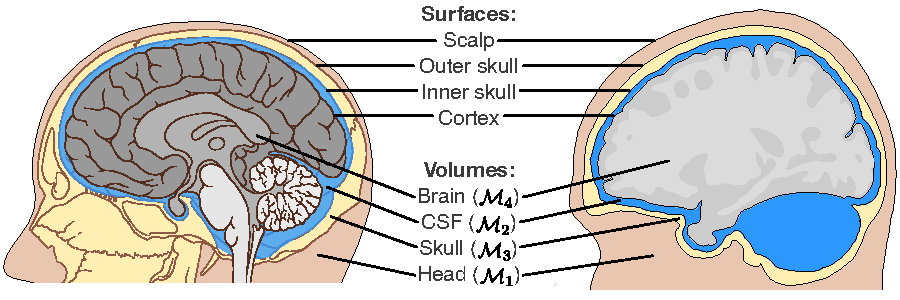
\includegraphics[width=\linewidth]{./img/HeadSurfacesVolumes}
\caption{Geometric domain defined by relevant tissues in the subject's head. The 4-sphere model considers three media: brain, cerebrospinal fluid (CSF), and the rest of the head. Relevant interfaces between media are displayed: brain cortex, inner and outer skull, and scalp. Notice the anatomical simplifications described in the text. (Left) Realistic illustration of a human head. Composition from two diagrams by Patrick L. Lynch and C. Carl Jaffe \cite{wikipic1, wikipic2}.  (Right) Cross-section of the surfaces obtained from the ICBM152 template after segmentation}
\label{fig:diagrams2}
\end{figure}

With the media defined formally, reflective boundary conditions can be written as follows,
\begin{equation}
\sigma(\rr)\, \nabla V(\rr) \cdot \mathbf{n} = 0, 
\text{ for } \rr \in \mathcal{M}_1
\label{eq:boundary1}
\end{equation}
where $\mathbf{n}$ is a vector orthogonal to $\partial\mathcal{M}_1$.
%
At the interfaces between media, the boundary conditions are to have continuous first derivatives; this property can be requested for the whole domain,
\begin{align}
    V\ppar{\bullet}, \sigma\ppar{\bullet} V\ppar{\bullet}  
    &\in C^1\ppar{\mathcal{M}_1 \cup \mathcal{M}_2 \cup \mathcal{M}_3 \cup \mathcal{M}_4 }
\end{align}

The continuity of $\sigma(\rr) V(\rr)$ is particularly important on the interfaces between media because the conductivity, $\sigma$, is expected to be homogeneous within each media but to change drastically between different media. 

To make sense of the magnitudes of the discontinuities of the conductivity, $\sigma$, among different media, in table \ref{tab:conductivity} are displayed typical values for the four media described before; data is from Ramon et al \cite{ramon2006influence}. See figure \ref{fig:diagrams2} for a visual reference of these tissues.

\begin{table}[]
\centering
\begin{tabular}{lr}
\toprule
Tissue              & Conductivity (\unit{\micro \siemens/\cm}) \\ 
\midrule
White matter        & 1.43         \\
Gray Matter         & 3.33         \\
Cerebrospinal Fluid & 15.38        \\
Skull Tissue        & 625.00       \\
Scalp               & 1.74        \\
\bottomrule
\end{tabular}
\caption{Conductivity for different head tissues considered in the Four-sphere model, measured in microsiemens per centimeter. Data from \cite{ramon2006influence}}
\label{tab:conductivity}
\end{table}

\subsection{Construction of the leadfield operator}

Recall that both equations \eqref{eq:poisson_gral} and \eqref{eq:poisson_isotropic} are constructed for one sensor and one dipole with unit magnitude.
%
We now consider a finite number of EEG sensors at locations $\sa_1, \sa_2, \dots, \sa_M \in \R^3$, and dipoles at locations $\dd_1, \dd_2, \dots, \dd_N \in \R^3$
with momenta $\mm_1, \mm_2, \dots, \mm_N$.
%
For ease of notation, write each momentum as
\begin{equation}
    \mm_n = \rho_n\, \ee_n
\end{equation}
with $\rho_n\in \R, \ee_n\in \R^3$ such that $\ee_n$ has unit norm, i.e. $\nnorm{\ee_n}_2 = 1$.

%
After making the assumptions described in the previous sections, we may conclude that the electric scalar field, $V$, is given by
\begin{equation}
V(\rr) = 
\sum_{n=1}^N \rho_n \tilde{V}_{n}(\rr)
\end{equation}
where $\tilde{V}_n$ is the solution to the following equation
\begin{equation}
\nabla \cdot\ppar{\sigma(\rr)\, \nabla \tilde{V}_n(\rr) } = 
{\delta\ppar{\rr-\dd_n^+} - \delta\ppar{\rr-\dd_n^-}}
\end{equation}
under the boundary conditions from equation \eqref{eq:boundary1}, and with each $\dd_n^\pm$ constructed from $\dd_n$.
%
For ease of notation, define 
\begin{align}
g(\rr, \dd_n) &= \tilde{V}_n(\rr)
\end{align}
and thus, we can write
\begin{equation}
V(\rr) = 
\sum_{n=1}^N \rho_n\, g\ppar{\rr, \dd_n} = 
\begin{bmatrix}
    g\ppar{\rr, \dd_1} & 
    g\ppar{\rr, \dd_2} &
    \cdots &
    g\ppar{\rr, \dd_N}
\end{bmatrix}
\begin{bmatrix}
    \rho_1 \\ \rho_2 \\ \vdots \\ \rho_N
\end{bmatrix}
\label{eq:back1}
\end{equation}
%\begin{equation}
%V(\rr) = 
%\sum_{n=1}^N \rho_n g\ppar{\rr, \dd_n} = 
%\spar{g\ppar{\rr, \dd_1}, g\ppar{\rr, d_2}, \cdots, g\ppar{r, d_N}}
%\spar{m_1, m_2, \cdots, m_N}\trans
%\label{eq:back1}
%\end{equation}

Furthermore, by using the equation for all the sensor locations and stacking the results, we obtain the following vector equation
\begin{equation}
\begin{bmatrix}
V\ppar{\sa_1} \\
V\ppar{\sa_2} \\
\vdots \\
V\ppar{\sa_M}
\end{bmatrix}
=
\begin{bmatrix}
    g\ppar{\sa_1, \dd_1} & 
    g\ppar{\sa_1, \dd_2} &
    \cdots &
    g\ppar{\sa_1, \dd_N} 
    \\
    g\ppar{\sa_2, \dd_1} & 
    g\ppar{\sa_2, \dd_2} &
    \cdots &
    g\ppar{\sa_2, \dd_N} 
    \\
    \vdots & \vdots & \ddots & \vdots
    \\
    g\ppar{\sa_M, \dd_1} & 
    g\ppar{\sa_M, \dd_2} &
    \cdots &
    g\ppar{\sa_M, \dd_N}
\end{bmatrix}
\begin{bmatrix}
    \rho_1 \\ \rho_2 \\ \vdots \\ \rho_N
\end{bmatrix}
\label{eq:model3}
\end{equation}

Equation \eqref{eq:model3} can be rewritten as the following generic matrix equation
\begin{equation}
\Y = \G\, \SA
\label{eq:model4}
\end{equation}
where $\Y \in \R^{M\times 1}$ encodes the EEG measurements, $\SA \in \R^{N\times 1}$ encodes the dipoles' magnitude, and $\G \in \R^{M\times N}$ is a matrix known as the leadfield matrix, gain matrix, forward operator, among other names; $\G$ encodes the mixture of current density to form the scalar electrical field measured by EEG sensors.



If the dipole's orientation, $\ee_n$, is to be determined, we can consider each dipole as the sum of three dipoles parallel to some orthogonal directions. Such as in figure \ref{fig:diagrams3}, we can write
\begin{equation}
\rho_n \ee_n = \rho^x_n \ee_n^x + \rho_n^y \ee_n^y + \rho_n^z \ee_n^z
\end{equation}
with $\ee_n^x, \ee_n^y, \ee_n^z \in \R^3$ vectors with unit norm located at $\dd_n$ and parallel to the respective $x-, y-, z-$axis.
%

Under these new circumstances, equation \eqref{eq:back1} changes to
\begin{equation}
V(\rr) = 
\sum_{n=1}^N 
\spar{
\rho_n^x\, g\ppar{\rr, \ee_n^x} +
\rho_n^y\, g\ppar{\rr, \ee_n^y} +
\rho_n^y\, g\ppar{\rr, \ee_n^z}
}
\end{equation}
which can be written as a matrix equation such as \eqref{eq:model4}.

The overall effect of assuming unknown orientations are (1) the increase of the number of dipole magnitudes to be determined by a factor of 3, as well as the size of the leadfield matrix, and (2)
we need to compute the magnitude of these dipoles in order to recover the original interpretation.

\begin{figure}
\centering
%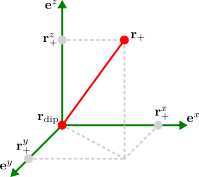
\includegraphics[width=0.4\linewidth]{./img_dev/OrthDecompOld}
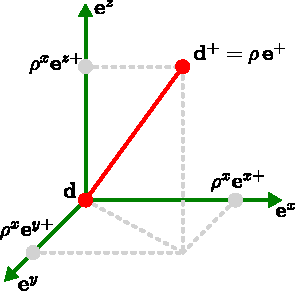
\includegraphics[scale=1.2]{./img/OrthDecomp}
\caption{Decomposition of a dipole with arbitrary momentum as a sum of dipoles whose momentum is parallel to their respective $x-, y-, z-$axis. By definition, a dipole is made of a sink and a source with equal charges. For visual simplicity, only the source $\mathbf{d}^+$ is shown; the sink $\mathbf{d}^-$ can be constructed similarly}
\label{fig:diagrams3}
\end{figure}

The forward model summarized in equation \eqref{eq:model4} can be extended trivially to account for $T$ EEG measurements in time by setting $\Y \in \R^{M\times T}$, $\SA \in \R^{M\times T}$, and $\G$ unchanged.
%
This is possible due to the quasi-static Maxwell equations. 
%
Since the neural electric fields change in time at relatively low frequencies, they don't induce an important change to the magnetic field \cite{nunez2006electric}.
%
The magnetic fields produced by the electric potentials can be considered constant, and thus, any capacitance can be neglected.

It is important to acknowledge that the changes in the electric and magnetic fields are independent of biological tissue.
%
However, the neural events that generate electrical fields also generate magnetic fields, which can be measured using Magnetoencephalography (MEG).

The quasi-static properties of the system imply that the magnetic and electric fields don't interact with each other.
%
Any correlation between them comes from their neural generators.
%
A complete discussion of this phenomenon is beyond the scope of this work.


\begin{comment}
\section{Limitations of surface electrodes}

There are several neural activity patterns that surface electrodes cannot represent properly.
%
Silent activity refers to neural activity that doesn't produce a significant electric potential and is not registered by surface electrodes.
%
It is estimated that only 20\% of the brain's energy is spent producing non-silent activity.

The orientation of neuron dendrites, which carry the post-synaptic potentials, is crucial in how much of their activity is actually recorded by surface electrodes.
%
Pyramidal neurons at the gray matter (located at the outer cortex) are almost exclusively oriented parallel to the cortex surface.
%
This common orientation, combined with their physical proximity to the scalp, makes the pyramidal neurons to be over-represented on recordings from surface electrodes.

On the other side, neural activity occurring at the lower layers of the brain is more difficult to register and reconstruct.

These limitations of this recording modality are inherited from the ESI methods, and thus, they must be considered when interpreting the obtained results.

A second set of limitations from the distributed dipole model represents a spatial average of the .
%
Distributed dipoles can efficiently represent synchronous activity over large regions, a phenomenon known as a source patch.
%
Distributed dipoles of low magnitude may represent smaller source patches and regions with asynchronous orientations, resulting in .




%
The distributed dipole model is agnostic in that it doesn't make any assumptions about the location of the dipoles.
%
A region with no active dipoles leads to equivalent dipoles with zero magnitude, while a region with active dipoles leads to equivalent dipoles with non-zero magnitude.
\end{comment}

\section{Practical considerations}

\subsection{Geometry Identification from Data}

Recall that the construction of the leadfield matrix, $\G$, is based on solving the equation \eqref{eq:poisson_gral} (or equation \eqref{eq:poisson_isotropic} in the isotropic case) 
subject to the boundary conditions in \eqref{eq:boundary1}.

These equations can be solved numerically using Boundary Element Methods (BEM) or Finite Element Methods.
%
A full review of these methods --even in the particular case of ESI-- is beyond the scope of this work, and the interested reader may refer to the review by Hallez \cite{hallez2007review} or that by Vorwerk et al \cite{vorwerk2012comparison}.

Needless to say, these methods are implemented in commercially available software such as OpenMEEG \cite{gramfort2010openmeeg}, DUNEuro \cite{schrader2021duneuro}, and MNE Python \cite{GramfortEtAl2013a}.

In this section, the goal is to describe the identification of the tissue media from an operative standpoint.
%
Tissues are often defined from the subject's anatomical data or an appropriately matched template.

The anatomical data often originates as the result of T1 or T2 magnetic resonance imaging (MRI) from the subject. 
%
Later, the MRI images are segmented: relevant tissues are identified, and triangulated 3D surfaces are constructed from them. 
%
Relevant algorithms for these tasks are available on commercial software such as CAT12 \cite{gaser2022cat} and Fieldtrip \cite{oostenveld2011fieldtrip}.

It is relevant to mention that the Fours Sphere model is not the only option for constructing the leadfield matrix. 
%
For instance, the model can be trivially extended to include five media by separating the brain into gray matter and white matter.
%
Such division requires a robust algorithm to distinguish between those tissues; since the interface is known to be non-smooth, robustness is a strong requirement.

\subsection{Location of Distributed Dipoles}

Over the previous sections, the locations of the distributed dipoles, $\mathbf{d}_n$, were assumed to be known.
%
Two cases were considered: if their orientation, $\mathbf{m}_n$, was assumed to be known or not.

Formally, the goal of ESI is to gain knowledge from the neural sources of electrical activity, including their location. 
%
Thus, we shouldn't make assumptions about their location.

In that sense, the most inclusive assumption is that the dipoles should be located `anywhere' inside the brain.
%
This assumption can be enforced by setting the locations of the distributed dipoles over a grid covering the entire brain volume.
%
In figure \ref{fig:dipoles}, two of these arrangements are displayed: a cubic grid and an adaptive grid. 
%
The adaptive grid, as implemented on the Brainstorm software \cite{brainstorm}, is constructed following these steps:
\begin{enumerate}
    \item Use cortex as initial layer.
    \item Downsample to locate dipoles with prescribed distance between them.
    \item Shrink to obtain next layer.
    \item Repeat until no more layer can be constructed.
\end{enumerate}
%first building multiple surfaces are constructed by shrinking the outer surface (cortex) and setting the dipoles over the obtained surfaced.

Adaptive grids offer some advantages since they are conceptually consistent with depth weighting (see section \ref{sec:wMNE}), and they can be constructed so that the outer layer falls within a certain distance from the cortex.

\begin{figure}
\centering
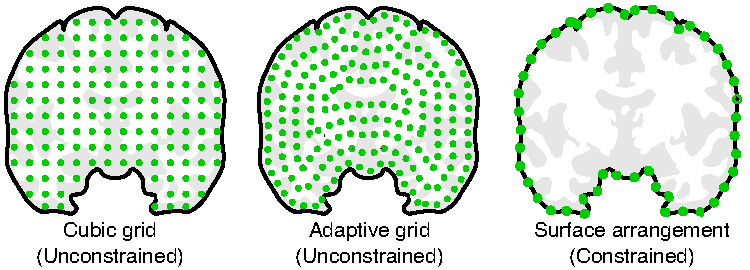
\includegraphics{./img/DipoleGrid.pdf}
\caption{Some configurations for distributed dipoles. Constrained dipoles have a known orientation (orthogonal to the cortex surface), while unconstrained dipoles have an unknown orientation.}
\label{fig:dipoles}
\end{figure}

In certain scenarios, the assumption of a total lack of information may be replaced by the assumption that the dipoles are located in the cortex and are oriented orthogonally to it.
%
This is justified by the peculiar geometry of the outer layers of the gray matter, which consist of neuron dendrites orthogonal to the cortex surface.
%
In figure \ref{fig:dipoles}, we may observe an arrangement of distributed dipoles that encodes this assumption.

Whether we may or not assume that the dipoles are located only in the cerebral cortex depends on additional assumptions of the neural processes under study.
%
Many `higher' cognitive processes are known to occur in the cerebral cortex: speech generation and recognition, face recognition, and spatial orientation, among others \cite{Saladin_Gan_2020}.
%
Conversely, we may ignore some deeper brain regions if their associated neural functions are not part of the phenomenon under study.

Many software dedicated to ESI refers to the case when dipoles are orthogonal to the cortex surface as `constrained,' while the other case is `unconstrained.' 
%
Other setups are possible, yet their discussion is outside the scope of this work.

\section{Conclusion}

\begin{comment}

\section{Extensions of the model}

The 4-sphere model is a prevalent standard in the modern literature.
%
Segmentation algorithms for the relevant tissues are available in many commercial software.

Different authors have addressed a number of limitations of the 4-sphere model.

For instance, extending the 4-sphere model into 5 spheres has been proposed by distinguishing between white matter and gray matter inside the brain.
%
The resulting model is almost identical, and the additional computational cost is not very large. 
%
However, the gray and white matter are very similar when observed using T1 MRI, even under normal conditions, and thus, very robust segmentation algorithms are required.

The assumption of isotropic conductivity has also been questioned.
%
Conductivity can be estimated using, for example, Diffusion Tensor Imaging.
%
[] investigated the benefits of including such additional information and concluded that anisotropic information should be used when available, but the enhancements do not justify the additional costs.

On the other hand, more simplistic models have also been proposed.
%
The Corrected 4-sphere model, for example, uses four spheres instead of volumes obtained from the subject.
%
TODO[ add comment]

Now, the 4-sphere model can be generalized to other types of electrical recordings.
%
For example, [] have used () to model intracranial electrodes, i.e., electrodes placed at the cortex surface or inside the brain.

In Chapter 3 we use the 1-sphere model to locate sources. 
\end{comment}
